\documentclass[a4paper, 12pt]{article}
\usepackage{a4wide}
\usepackage{textcomp}
\usepackage{listings}
\usepackage{color}

\usepackage{graphicx}
\graphicspath{ {./images/} }

\usepackage[backend=biber,style=numeric]{biblatex}
\addbibresource{bibliography.bib}

\definecolor{dkgreen}{rgb}{0,0.6,0}
\definecolor{gray}{rgb}{0.5,0.5,0.5}
\definecolor{mauve}{rgb}{0.58,0,0.82}

\lstset{frame=tb,
  language=Java,
  aboveskip=3mm,
  belowskip=3mm,
  showstringspaces=false,
  columns=flexible,
  basicstyle={\small\ttfamily},
  numbers=none,
  numberstyle=\tiny\color{gray},
  keywordstyle=\color{blue},
  commentstyle=\color{dkgreen},
  stringstyle=\color{mauve},
  breaklines=true,
  breakatwhitespace=true,
  tabsize=3
}

\begin{document}

    \title{A Graphical Programming Language Editor}
    \author{Candidate No. 198719}
    \date{Final Year Project}
    \clearpage\maketitle
    \thispagestyle{empty}

    \newpage\clearpage\thispagestyle{empty}
    \tableofcontents
    \newpage
    \setcounter{page}{1}

    \section{Introduction}
    Graphical programming can be a fantastic and intuitive way to introduce new programmers to
    the scene. When programmers ask others for assistance, those helping typically do so in a visual 
    style, using whiteboards, drawing flowcharts, with boxes and arrows indicating the flow 
    of the program. Why can't we make programs in the same style if we find it so helpful to read? 
    The concept behind graphical programming is specifying the elements of the program graphically 
    rather than textually~\cite{dehouck2015maturity}.

    Popular examples of graphical programming include Scratch, as well as a personal favourite that 
    I used during my GCSE Computing education, App Inventor!
    What's clever about Scratch is its simplicity due to the block-based visual programming, aimed 
    towards younger children to help them get into coding!

    \begin{figure}[h]
        \centering
        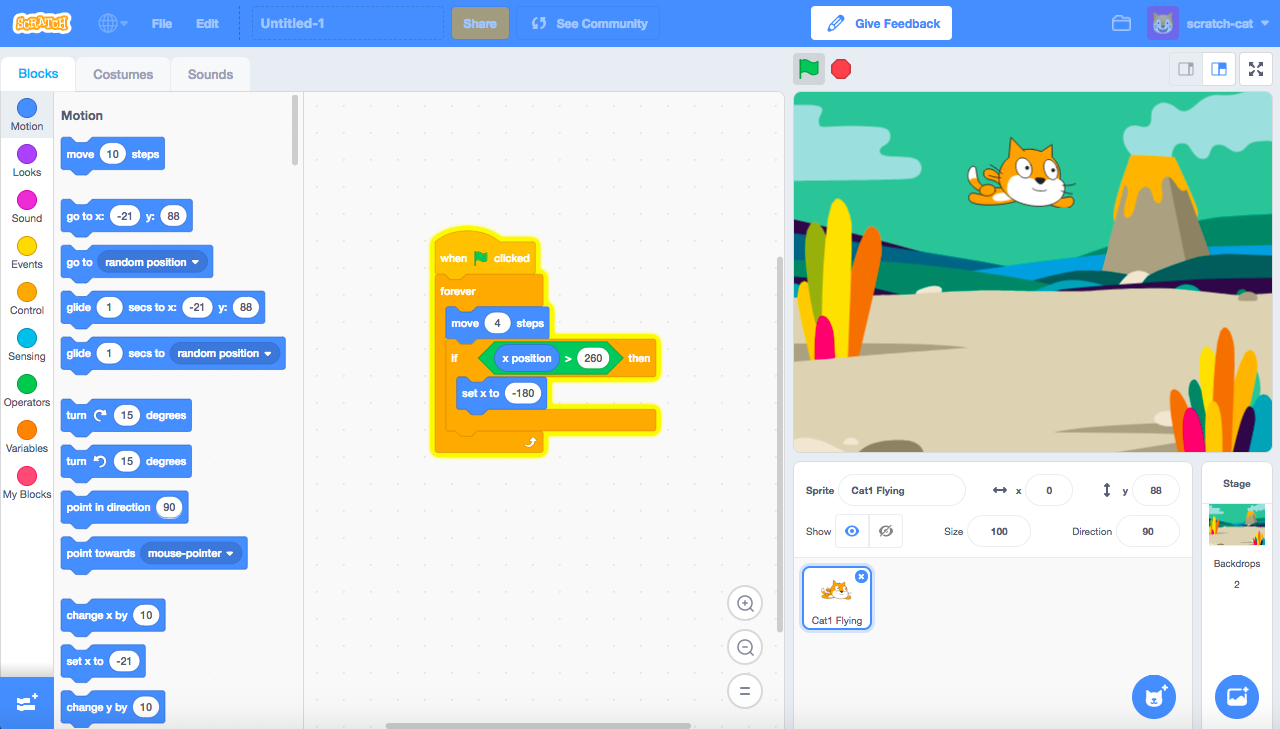
\includegraphics[width=160mm]{scratch_image}
        \caption{Scratch's visual scripting over a white canvas~\cite{thescratchteam}.}
    \end{figure}

    \clearpage
    MIT App Inventor is one of my personal favourites after experiencing it myself during GCSEs, 
    having to building an on-campus application for a University! It uses a graphical user 
    interface, similar to Scratch, as well as providing the blocks that you can use, visible on 
    the left hand side.

    \begin{figure}[h]
        \centering
        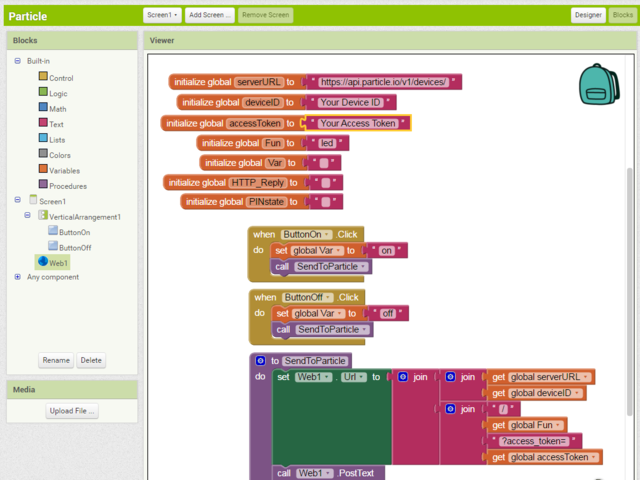
\includegraphics[width=150mm]{app_inventor}
        \caption{MIT App Inventor graphical programming~\cite{adafruit}.}
    \end{figure}

    Both what Scratch and App Inventor do superbly is colour code their blocks to identify 
    exactly what they are representing. There are colour coded blocks for variables, events 
    and controls, and so on! For instance in App Inventor, variables are coloured in Orange 
    blocks, and procedures and show in a big purple block, encapsulating all the blocks like 
    a function.

        \subsection{Aims}
            The aim of this project is to design and implement a simple interface for the
            user to graphically program basic functions. Simple functions may include:

            \begin{itemize}
                \item loops.
                \begin{itemize}
                    \item this includes \texttt{for} and \texttt{while} loops.
                \end{itemize}
                \item conditional statements, such as \texttt{if} statements.
                \item variables!
                \item arithmetic expression.
                \item print statements.
            \end{itemize}
            
            This is necessary as it provides another programming viewpoint for the user,
            which can aid them understand the process and flow of how said program may
            be running. It is also friendly and less intimidating for newer users,
            relative to a textual/command line script.
            
            I am going to program this is Java, my most experienced language, making use
            of Java's smart GUI design feature, whilst learning and building knowledge on
            said feature for my own experience.

        \subsection{Objectives}
            The main objectives are:

            \subsubsection{To investigate software requirements to produce a requirements
            specification.}
                It is important to clarify what the software requirements are for this project as they
                define whether this project will work or not. Without the mandatory requirements,
                the game will not be properly functional. I investigated what requirements are mandatory
                by doing research on existing softwares such as App Inventor and Blockly. For instance,
                all softwares I found had a \texttt{run} button in order to be able to run the graphical
                entities. Without this, how else is the canvas run? Of course it is not a big deal, and
                there would probably be another solution, but it's a simple feature that also provides
                simple UI for the user, which is self explanatory.

            \subsubsection{To select and justify an appropiate simple design for the
            project.}
                This objective is to research other designs of similar projects and to understand
                why their interface works well from a new user's perspective, but also why it
                doesn't work very well. My knowledge in Human-Computer Interaction will help me
                to focus on the design, and what defines a \textit{"user-friendly"} design.
                The goal here isn't implementing the design, it's creating a design, on pen paper,
                attempting to make it as self-explanatory as possible. But that also begs the question,
                \textit{"what determines a self-explanatory design?"} It's important to realise that
                everyone's judgement of what a simple design looks like is different. It's a subjective
                topic but I must ensure I use the principles learnt from HCI about simple design and
                user-friendly interaction to make a design at the best of my ability.
            
            \subsubsection{Implement a simple interface for users which is easy to
            understand.}
                An important objective, which builds off of \texttt{1.2.2}. I have limited GUI
                experience, where the first and last GUI building I engaged with was in 2nd year,
                Further Programming module, with Dr. Ian Wakeman. I spent a lot of time during that
                assignment at the time focusing on a simple interface for the Futoshiki puzzle.

                This objective will benefit me greatly. Through research and problems, I will
                get through this objective and implement an interface, whether it be outstanding,
                or just about finished, and I will gain a lot of knowledge and experience on
                the way.

            \subsubsection{Functional and working loops, conditionals and
            variables that can be interacted with.}
                What's the point of having a pretty canvas if you can't do anything with it?
                This is the meat of the project, what's going to make the project be useful.
                The main objective here is this one. My main priority is the ability to get
                this project off its feet.

                Variables for user's to be able to create and store data with, as well as
                interact with within the project. Loops to allow the user to work with logic.
                Without this objective being met, it's just a pretty GUI with no functionality.

        \subsection{Problem Area}
            The main challenge of implementing an interface to be able to program on is the required 
            time and skill set. This project may never be fully complete as more work can always be 
            done to improve the functionality of the interface, or making the interface more user-friendly.

            The project can be broken down into key areas that require focusing on:
        
            \begin{itemize}
                \item Graphical Design - modelling, interface, simplicity, GUI.
                \item Functionality - programming.
            \end{itemize}

            I have limited GUI design in Java from my 2nd year module, Further Programming, therefore this 
            process can be said to take up a large amount of time. Careful consideration is needed to 
            not overspend my time on the GUI design process, and rather get the functionality of said 
            interface to work.

            Functionality requires programming to be clean and efficient, so not to go back over the code 
            and forget what was written. Code must be documented and commented along the way to make sure 
            anyone who reads the code, including myself in the future, is able to understand what was 
            written and why it was decided.

            \subsection{Expected Outcomes}
            The expected outcomes of this project are a fully working, functional graphical programming 
            language interface. The user should use the tool independent from the back-end Java textual 
            code, and be able to perform the certain tasks:

            \begin{itemize}
                \item loops - create and work with basic for \& while loops.
                \item variables - create, store data and interact with variables.
                \item interface - an interface for users to be able to interact with and perform the
                above outcomes.
            \end{itemize}

            What do we expect it to behave/look like? A blank canvas should appear upon starting, with
            a heading on the left hand side, presenting the user with a selection of choice such as
            \textit{"Loops, Procedures"} and so on, for each category of block. They will be able to click
            on said heading, which will expand and show the different blocks they can choose from. So if
            they chose the \textit{loops} heading (a draft name for now, I know), this will expand and show
            for \& while loops for them to choose from.

            An important point to address, is what will happen when the user runs the program? This is a key
            concept which will be an ongoing investigation throughout the project. But the current idea is
            simple: an output screen showing the terminal. Upon running, a heading on the right hand side,
            or perhaps underneath, will pop out with the terminal showing you the output of your program.


            \subsection{Relevance}
            This project involves modules across my degree, as well as Java; the most extensively
            used language across my university education thus far. This project will use skills learnt
            in Human Computer Interaction; test my ability to understand the user's perspective and
            struggles, involving the evaluation of the software, rather than my own when designing
            the interface for them to use.
        
            This project also incorporates key concepts understood from Software Engineering.
            The ability to criticse my own work, collect requirements, manage time and manage an
            agile approach to the project. Therefore, this project will test my ability to make use
            of several skills in such a way that they will be used outside of my university education.

    \clearpage
    \section{Professional and Ethical Considerations}
        Below you will find the relevant sections of the BCS Code Conduct that apply to this 
        project. Since this project will not require any human participation, no ethical review 
        is necessary.

        \subsection{BCS Code of Conduct}
            \textbf{1.1 - have due regard for public health, privacy, security and wellbeing of others 
            and the environment;} \\\\
            This project does not feature any distressing visuals that may harm the user. \\\\
            \textbf{2.1 - only undertake to do work or provide a service that is within your professional 
            competence;} \\\\
            This project is within my professional skillset to complete. \\\\
            \textbf{2.3 - develop your professional knowledge, skills and competence on a continuing 
            basis, maintaining awareness of technological developments, procedures, and standards 
            that are relevant to your field;} \\\\
            Throughout this project I will maintain my skills, but further learn and research new ideas 
            or more experienced methods to make my skills more proficient within the field. \\\\
            \textbf{2.5 - respect and value alternative viewpoints and seek, accept and offer honest 
            criticisms of work;} \\\\
            I will accept feedback by my supervisor and others and use the criticisms to develop and 
            build upon the project further. Results of feedback will not be edited. \\\\
            \textbf{3.2 - seek to avoid any situation that may give rise to a conflict of interest 
            between you and your relevant authority;} \\\\
            Throughout the project I will be respect to my colleagues and my supervisor.

    \clearpage
    \section{Related Work}
        \subsection{Scratch}
            The key goal that Scratch sticks by is trying to introduce programming to those with no
            programming experience knowledge whatsoever. Scratch has been widely distributed to school
            systems and education organisations~\cite{maloney2010scratch}. Scratch also couldn't be any
            more clearer to use, with a heading of categories for you to choose and select the difference
            blocks that provide different functionality.

            \begin{figure}[h]
                \centering
                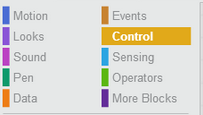
\includegraphics{scratch_blocks.png}
                \caption{Scratch's categories of blocks that you can select from.}
            \end{figure}

            The user doesn't require any documentation to understand how to use Scratch, rather they
            are able to learn on the go, hence why it is suitable to new programmers trying to get a
            basic feel of the approach and what programming can do, as well as what you are able to
            do with it!

        \subsection{MIT App Inventor}
            MIT App Inventor is another graphical programming language for building apps for Android devices.
            App Inventor is used across 195 countries, in education organisations and also self-taught
            \cite{xie2016skill}. 

            \begin{figure}[h]
                \centering
                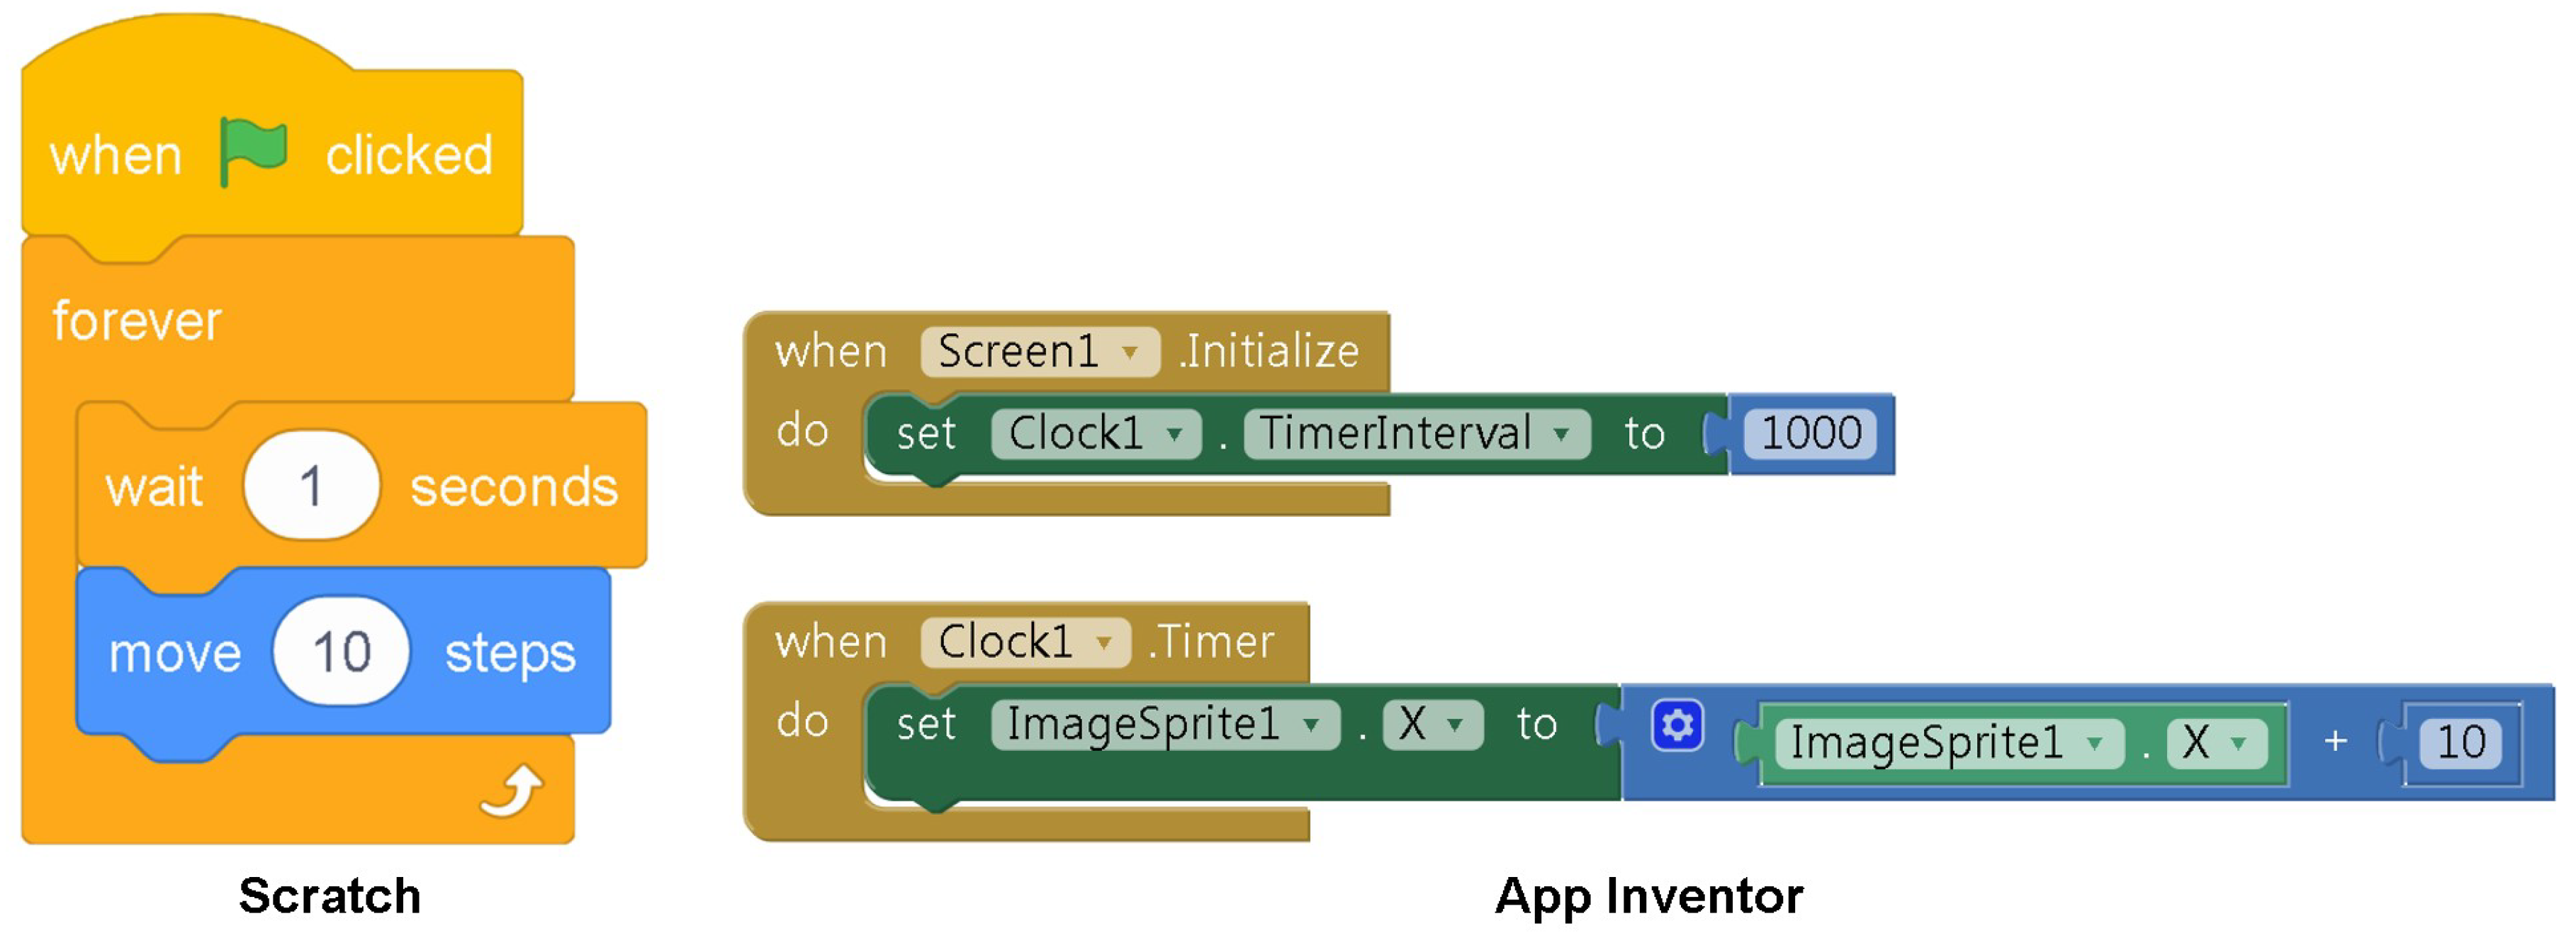
\includegraphics[width=125mm]{scratch_vs_appinventor.png}
                \caption{Graphical style of Scratch vs App Inventor~\cite{park2019comparing}. App Inventor is slightly more sophisticated.}
            \end{figure}

            \clearpage
            Scratch and MIT App Inventor are the two most widely used block-based graphical programming
            languages for students and/or pupils. As of August 2019, there were 44,981,198 registered
            users on Scratch, and 8,200,000 registered users on App Inventor~\cite{park2019comparing}.

            Both Scratch and App Inventor share the common goal of providing an educational programming
            language for new comers. Scratch is mainly used as a foundation to teach younger children
            the concepts of code, whereas App Inventor is used as the \textit{"step up"}, but both are
            used globally to make programming a bit more fun and interactive. App Inventor in particular
            is rewarding as upon running the code, an interactive mobile phone displaying your app is
            shown as the output!

        \subsection{Blockly}
            Blockly is probably by far the most modern out of the three I have proposed, and the 
            most intuitive. It's a free, web-based, open-source project by Google, built upon the 
            idea of Scratch. But what's intuitive about Blockly is the textual programming output 
            on the right-hand side of your graphical code. It can generate code in the following 
            languages~\cite{nbcbayarea}:

            \begin{itemize}
                \item Javascript.
                \item Lua.
                \item Dart.
                \item Python.
                \item PHP.
            \end{itemize}

            It can also be edited to generate code in a different textual programming language!

            \begin{figure}[h]
                \centering
                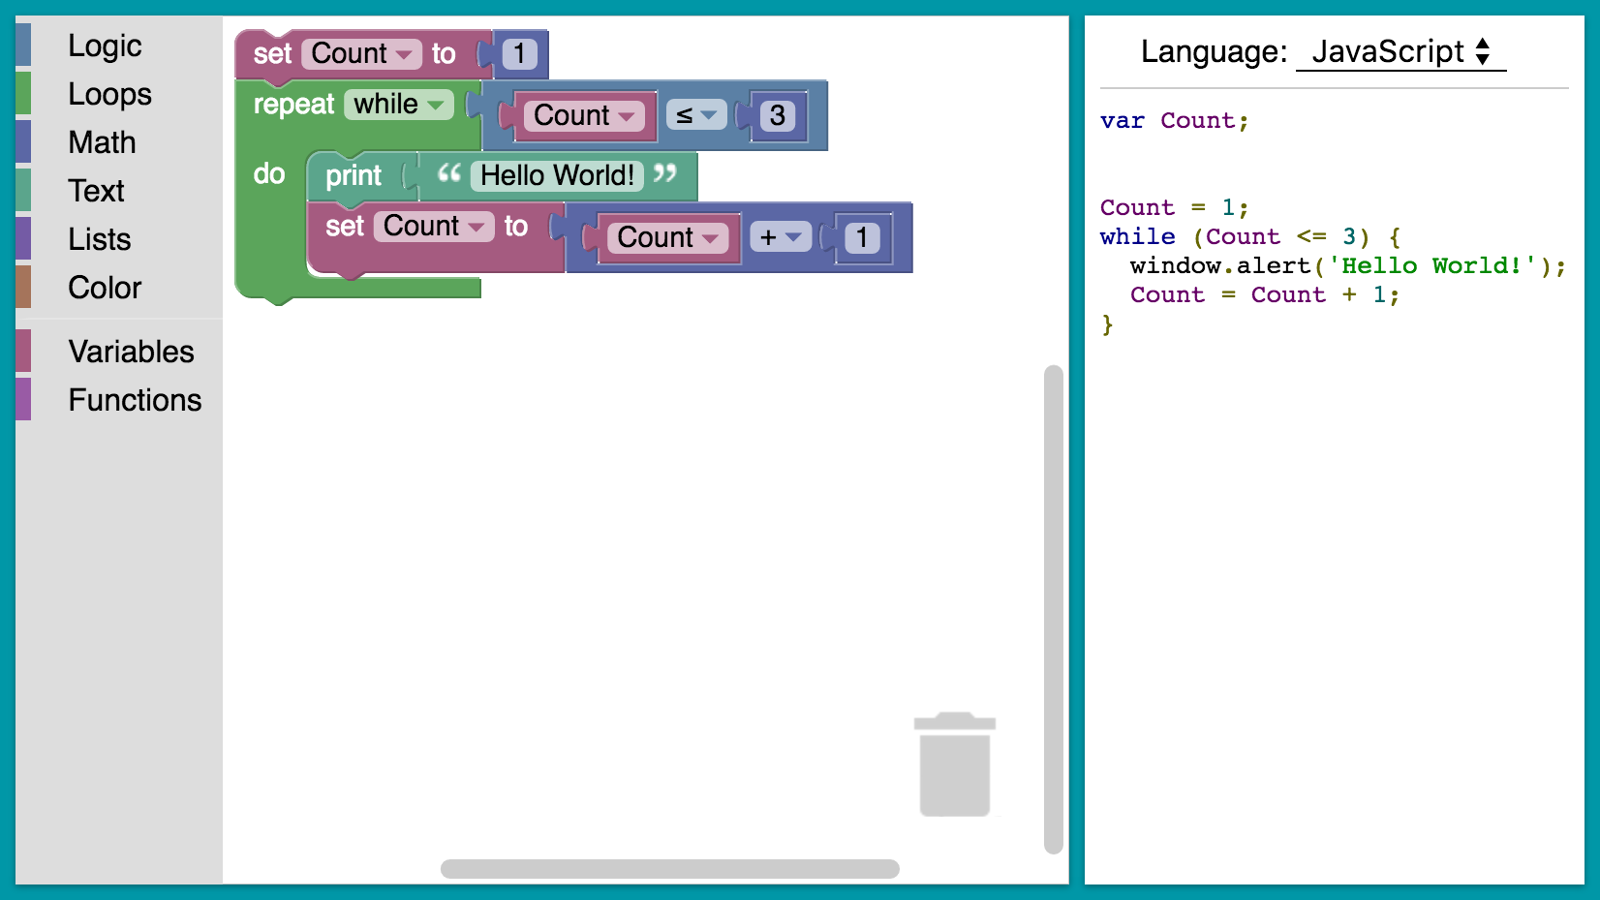
\includegraphics[width=150mm]{blockly.png}
                \caption{Blockly's modern and simple block programming design, as well 
                as the option to choose the programming language that it will syntactically 
                output as~\cite{blockly}.}
            \end{figure}

            Blockly is aimed towards new programmers to get them onboard and addicted to the visual 
            scene first. By providing the textual version of the code, perhaps this might spark a 
            passion within the user to follow through with programming. By being provided with the 
            textual code of their graphical app, they are learning and understanding what the code 
            will really look like and how they could potentially implement it themselves.

            A key part of Blockly that the developers undertook was user testing. The conditional and loop blocks were in the same category, with the same colour, 
            confusing the users who expected the program to run a certain way, when it ran differently 
            to what they were expecting ~\cite{fraser2015ten}. The developers understood this and 
            learnt from the feedback quickly, moving the conditionals to a different category, as 
            well as changing the colour too. This removed the confusion instantly. These key ways to improve 
            from feedback received is key to building a successful project.
        
        \clearpage
        \subsection{Graphical Programming}
            What all three graphical programming editors do together is follow the convention 
            of lower-case naming of variables, functions and so on that is followed in textual-based
            programming languages, for instance \textit{"if"} and \textit{"while"}. 

            \begin{figure}[h]
                \centering
                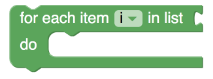
\includegraphics{lowercase_convention.png}
                \caption{The lowercase convention, as followed by Blockly as an example~\cite{pasternak2017tips}.}
            \end{figure}

            Graphical programming is not a permanent solution to programming, but rather an 
            introduction~\cite{gregoryvisual}. Users are being taught the convention of the key
            syntax that is used across all languages. I plan to follow this convetion too. A
            picture is worth a thousand words~\cite{petre1995looking}, and reading code isn't learnt
            nearly as fast and reading a picture. The strength of graphical representations is
            that they complement perceptually something also expressed textually in this case.

    \clearpage
    \section{Requirements Analysis}
        In this section, I have taken into careful consideration the aims and objectives for this
        project. Below you will find a compiled list of software requirements, split into two
        categories: \textbf{mandatory} requirements, the fundamental requirements that is needed
        for the project to work, and \textbf{desirable} requirements, optional further requirements
        that can be met to provide further quality of life experiences for the user.

        \subsection{Mandatory Requirements}

            \begin{table}[h]
                \begin{tabular}{|l|l|}
                    \hline
                    \multicolumn{2}{|c|}{\textbf{Mandatory Requirements}}                                                                                                                                                                                                             \\ \hline
                    \textbf{Requirement}                                                                                                     & \textbf{Specification}                                                                                                                 \\ \hline
                    \begin{tabular}[c]{@{}l@{}}1. Application will work on any java-run\\ environment.\end{tabular}                          & \begin{tabular}[c]{@{}l@{}}Whether the user is on a Windows, macOS\\ or Linux system, the application will work.\end{tabular}          \\ \hline
                    \begin{tabular}[c]{@{}l@{}}2. The interface shall accept user input\\ via keyboard and mouse.\end{tabular}               & \begin{tabular}[c]{@{}l@{}}User will be able to use keyboard and mouse\\ to create and interact with the canvas.\end{tabular}          \\ \hline
                    3. The program shall run until is it killed.                                                                             & \begin{tabular}[c]{@{}l@{}}The process will not stop running until either\\ it is killed via user or forced shutdown.\end{tabular}     \\ \hline
                    \begin{tabular}[c]{@{}l@{}}4. The program will output any errors,\\ if any.\end{tabular}                                 & \begin{tabular}[c]{@{}l@{}}If there are any run-time errors, the terminal\\ will output those for the user to see.\end{tabular}        \\ \hline
                    \begin{tabular}[c]{@{}l@{}}5. The user shall be able to use functional\\ loops such as for and while loops.\end{tabular} & \begin{tabular}[c]{@{}l@{}}The user will have the ability to interact with\\ loops in the interface.\end{tabular}                      \\ \hline
                    \begin{tabular}[c]{@{}l@{}}6. The user shall be able to create\\ variables.\end{tabular}                                 & \begin{tabular}[c]{@{}l@{}}The user will be able to create and interact\\ with variables.\end{tabular}                                 \\ \hline
                    7. A run button.                                                                                                         & A button to run to be able to run their program.                                                                                       \\ \hline
                \end{tabular}
            \end{table}

        \clearpage
        \subsection{Desirable Requirements}
            \begin{table}[h]
                \begin{tabular}{|l|l|}
                    \hline
                    \multicolumn{2}{|c|}{\textbf{Desirable Requirements}}                                                                                                                                                                                                                                                                           \\ \hline
                    \textbf{Requirement}                                                   & \textbf{Specification}                                                                                                                                                                                                                                 \\ \hline
                    1. Colour coded blocks.                                                & \begin{tabular}[c]{@{}l@{}}The designs can be colour coded to visually\\ aid the user what they represent. For instance,\\ orange blocks for variables.\end{tabular}                                                                                   \\ \hline
                    2. Interactive sound design.                                           & \begin{tabular}[c]{@{}l@{}}A potential sound that can be producing by\\ interacting with the program. For instance,\\ dragging and dropping, clicking, etc...\end{tabular}                                                                             \\ \hline
                    \begin{tabular}[c]{@{}l@{}}3. Highlight when mouse\\ over\end{tabular} & \begin{tabular}[c]{@{}l@{}}When the mouse is hovered over an object,\\ said object could be highlighted by a glowing\\ fade, or perhaps an outline of the object.\end{tabular}                                                                         \\ \hline
                    4. Recycling bin.                                                      & \begin{tabular}[c]{@{}l@{}}A recycling bin in the bottom corner to show\\ users where they can drag and drop blocks\\ that are not needed. This could only be visible\\ when an object is being dragged, or it could always\\ be visible.\end{tabular} \\ \hline
                    5. Undo button.                                                        & A button to undo an action.                                                                                                                                                                                                                            \\ \hline
                    6. Redo button.                                                        & A button to redo an action if undone.                                                                                                                                                                                                                  \\ \hline
                \end{tabular}
            \end{table}

        My aim is to attempt to achieve all the mandatory requirements as they are underlying
        foundations of the program. All the requirements work together to build the program. 
        Without any of these requirements, this will fail to work effectively. The desirable 
        requirements that I would like to be able to implement include the undo + redo button, 
        as well as the recycling bin! Thinking about the user's goals here, these would be 
        incredibly impactful towards benefiting their quality of life experience. Having the 
        ability to undo/redo any mistakes you make, as well as simply drag and drop to the bin 
        to delete unnecessary content, only makes the lives of the user easier.

    \clearpage
    \section{Project Plan}
        Below in figure 7 is a gantt chart outlining my process to progress through this task.
            
        \begin{figure}[h]
            \centering
            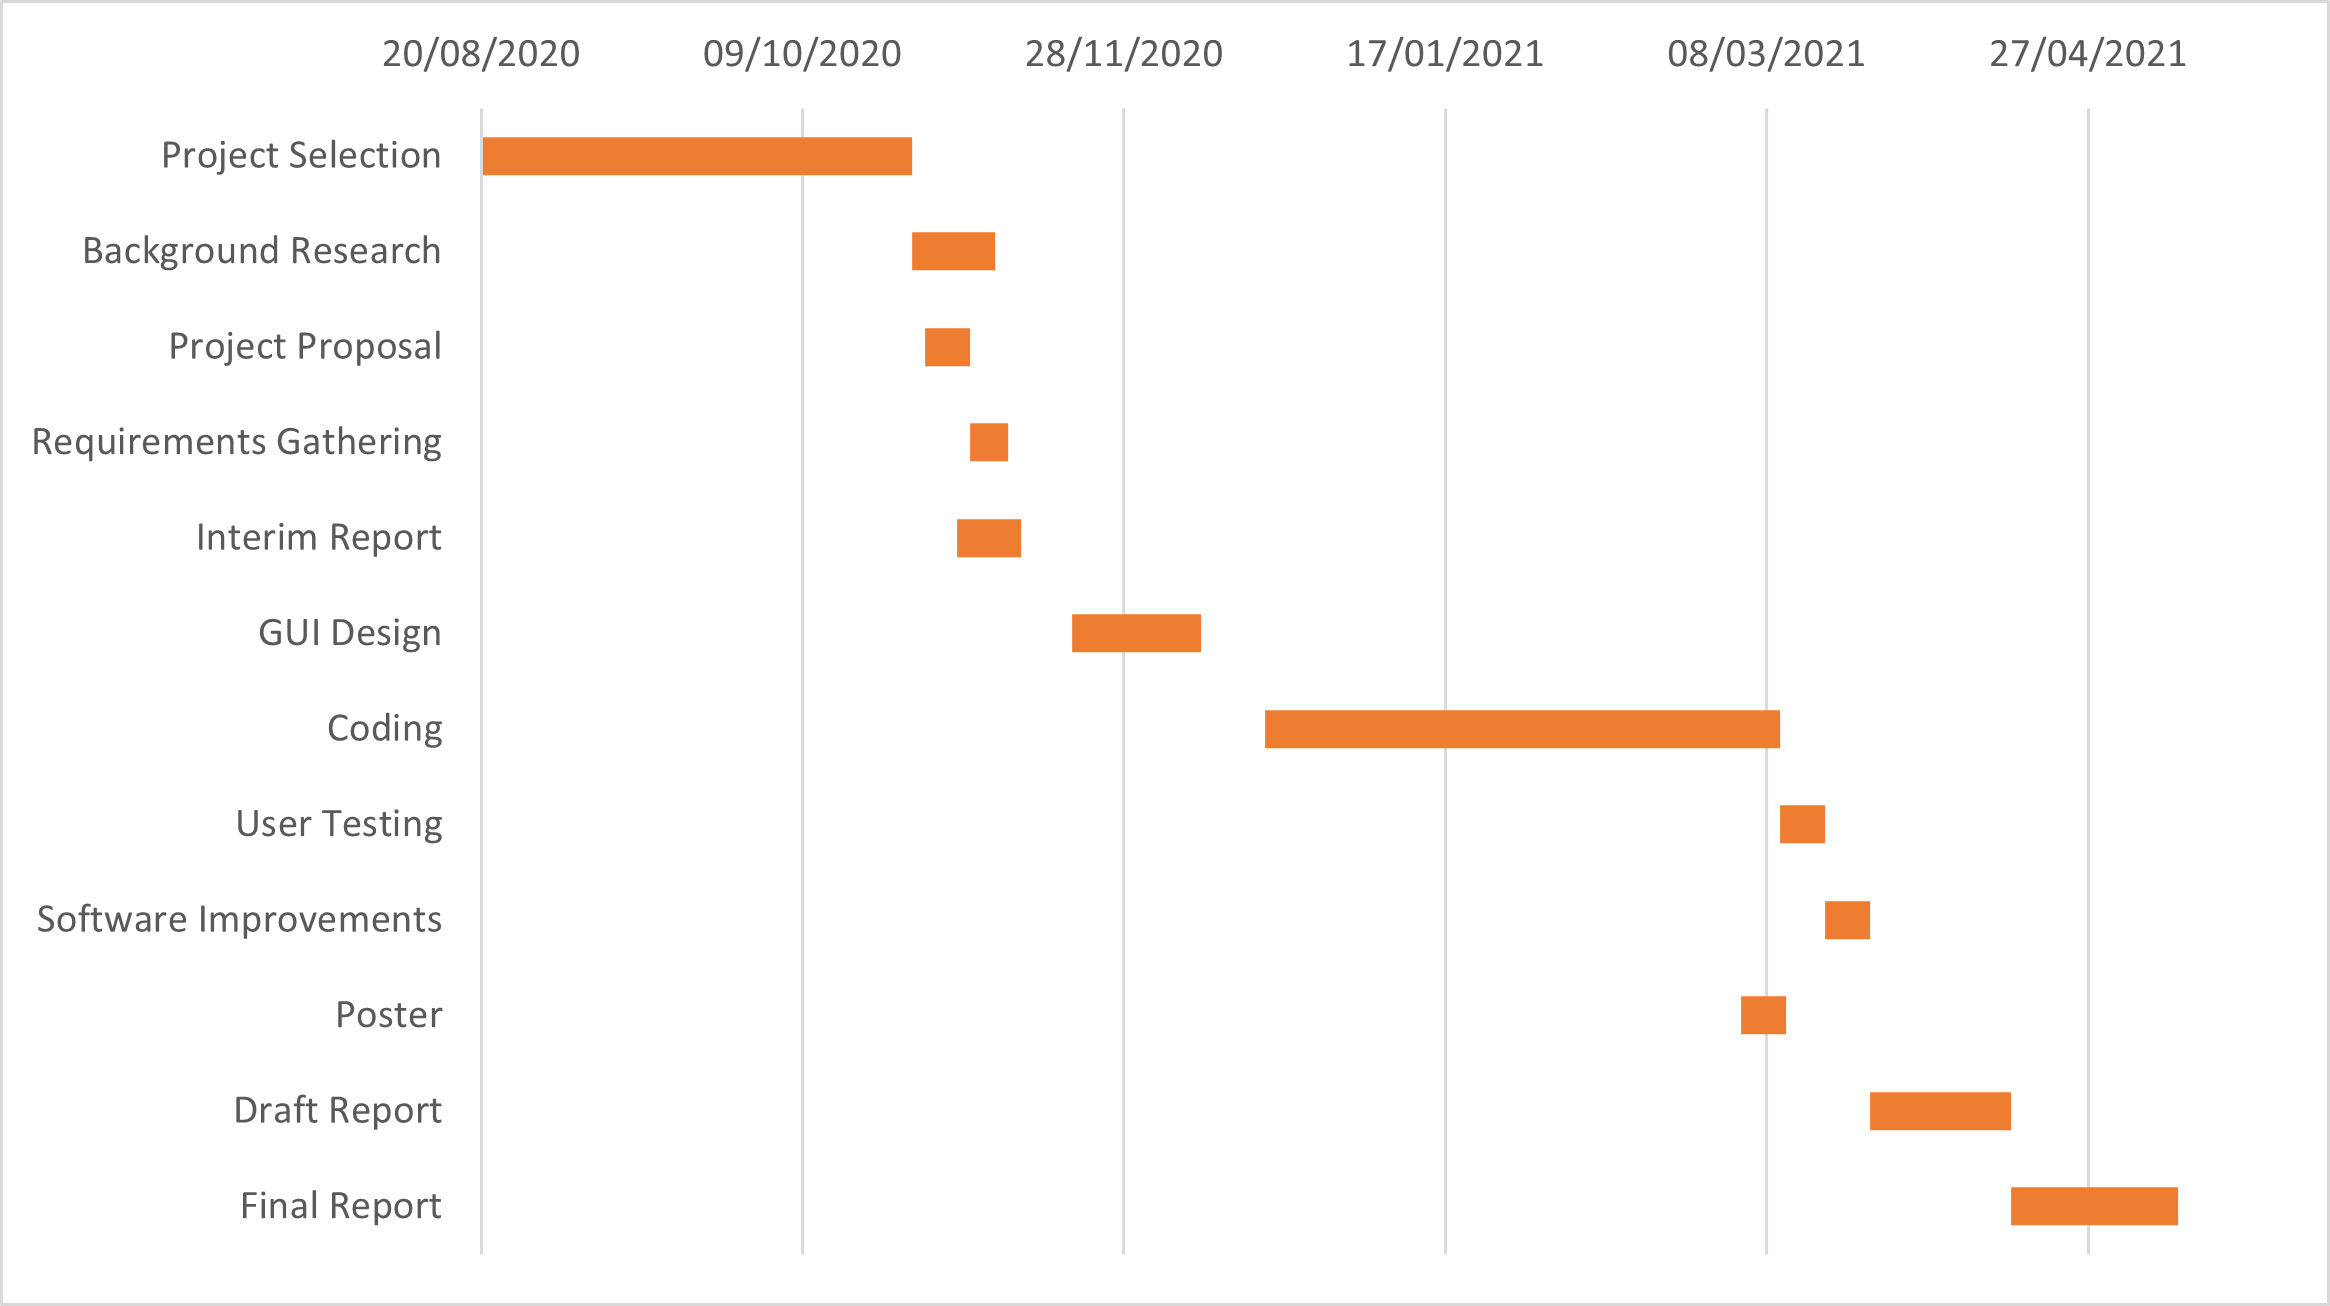
\includegraphics[width=150mm]{gantt_chart.png}
            \caption{My gantt chart displaying the process I intend to follow throughout
            the project.}
        \end{figure}

        \subsection{Completed Work}
            As of the time of this report being handed in, all the work I have completed thus
            far are the following:

            \begin{itemize}
                \item Project proposal - outlining my objecives, aims and motivations for the
                project.
                \item Background research - related work to the project I am working on.
                \item Requirements gathering - software requirements that must be met for
                the project to work, as well as some desirable objectives for quality of
                life improvements!
                \item Interim report.
            \end{itemize}

        \subsection{What's to come}
            After completing this, I plan to have a meeting with my supervisor soon to discuss
            design ideas for the project, and what the GUI might potentially look like.

            Of course, throughout the project my draft report will be the main task. Although
            my gantt chart shows a period in March-April where I will be hard focusing on it,
            throughout the project, I do plan to add bits here and there to it, to get started.

        \subsection{Other Tools}
            I have utilised a private Github repository for version control.

            \begin{figure}[h]
                \centering
                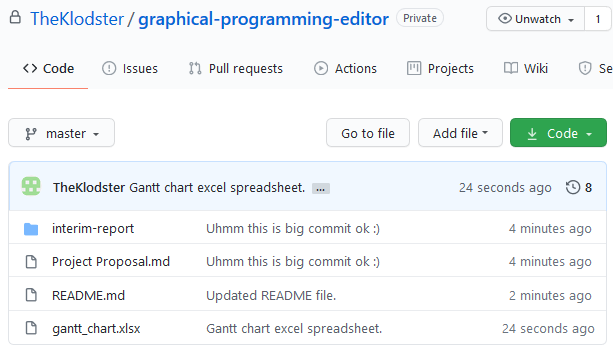
\includegraphics[width=110mm]{github.png}
                \caption{My Github private repository for the project.}
            \end{figure}
    
    \clearpage
    \section{Main Report}
        \subsection{Designing a rough GUI}
            What I do at the beginning of this project is crucial to what will come up ahead since this
            will be the foundation of the entire project. How I will present the work to the user. Before
            I can begin getting into the deep fundamentals of this project, I must first, but most
            importantly of all, design the basic canvas GUI (graphical user interface) for the user to
            be able to see! This initial design of this interface will be a blank canvas, hopefully
            with a left-hand side panel where the blocks will be. \\

            To begin, I will start with the blank canvas, then leading onto dividing the canvas into two
            so there is a left side panel, and in this panel, a print block that the user will be able
            to drag and drop. The functionality will not matter currently at this stage, but it's
            essential I research how I will implement the blocks, as this is the commitment I will need
            to take for the rest of the project. I will start with making the blocks out of buttons.
            I should note that the reason the start of this project is the most important and requires
            careful thought and consideration is simply that this is not a small project. I must
            ensure that whatever I do now will work for the remainder of the project, and that it will
            be compatible with any functionality I will implement later. If I don't consider this
            carefully, there may be a chance that I might hit a dead end and I will have to come back
            to this stage, at a time where I shouldn't be. \\

            Upon building basic GUI upon running the program, it would be nice if it was centered so it
            can be visible on any resolution that the user will be using. Thinking it would be a simple
            case of researching the Java JFrame documentation, I did not find what I was looking for and
            branched out. \textit{Jack} from this thread about setting up JFrames to the centre of the
            screen regardless of resolution provided an excellent function which takes the resolution of
            the screen and mathematically applies divisions so that it will be centred of any screen
            resolution we use \cite{jackSO}. Figure 9 shows a rough sketch about the idea I have for what the interface will roughly look
            like. This may change in the near future when I begin implementing the JPanels, but for now
            this sort of design would look appropriate and make sense for the user. This type of formation
            is adopted too by other applications such as Scratch and App Inventor - both use a design
            similar to this where the control panel is on the left hand side with all the different
            blocks the user can use, followed by the big canvas in the centre. \\


            Upon implementing the buttons I had them hugging the sides of the button panel, which didn't
            look appealing at all, so I had a read through the BorderLayout documentation which revealed
            that I could enter some padding to sort out the issue.

            \clearpage
            \begin{figure}[h]
                \centering
                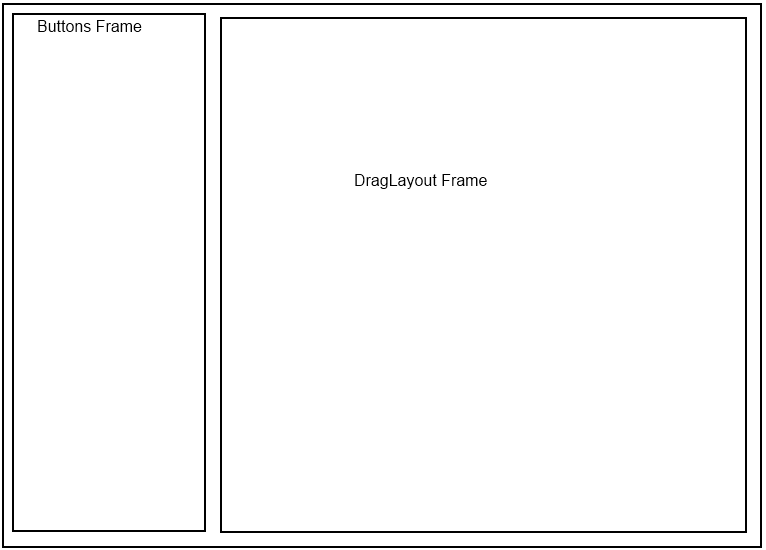
\includegraphics[width=120mm]{design.png}
                \caption{Drawn out plan on essentially what the interface may look like, subject to change.}
            \end{figure}

            In regards to the console output for the user, I could do this several ways. A particular way
            I had in mind specifically was to research whether Java Swing could be able to open another
            window showing the output as a result of running the user's program. This is not the focus
            for the time being, so more on this later. Furthermore, I didn't want the user to be able
            to resize the program as this could potentially lead to issues in the GUI not showing the
            user all the information they need to work, or not giving them enough space - a simple
            \texttt{frame.setResizable(false);} worked like a charm. \\

            I ran into a problem whereby in Java Swing, when I added padding to the border edges that
            are touching the edges of the JFrame, the background colour filled outside the border. \\

            \clearpage
            Firstly, the background of the panel is painted. Then the border is painted afterwards
            - weather a compound border function is used where the function allows you to
            specify the border objects for the outside and inside edges. Secondly, then the border
            is painted on top of the panel. In the case of my panels, only the line is painted on
            top of the background. I will be used a compound border to adjust the margins for the
            borders around the panels. I will run into this issue where the white background colour
            I choose will overflow. \\

            \begin{figure}[h]
                \centering
                
\includegraphics[width=80mm]{colour_overfill.png}
                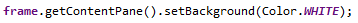
\includegraphics[width=100mm]{overfill_solution.png}
                
\includegraphics[width=80mm]{no_overfill.png}
                \caption{The white background overflowing above the border in the top image; my solution
                to the current problem, and the gray background now just appearing as a white background.
                No one liked a gray background anyway.}
            \end{figure}
        
        \clearpage
        \subsection{Copy Constructor}
            The procedure forward is to design the application only using a print statement. Upon
            succeeding with said functionality, the follow up for the remainder of the implementations
            would function more or less the same, and it should be an easy job of copy and paste.
            I created a button named \texttt{print statement} that would be the button used to initialise
            a print statement.The next important step was reproducing this in the main canvas panel.
            I implemented functionality that listens to the mouse clicks, thus once the button is
            pressed, it clones it on the canvas to be used. Initially I was going to implement the
            \texttt{Cloneable} library but I came across an article that suggested otherwise.
            \texttt{Cloneable} is broken and shouldn't be used as the architecture was essentially
            mistaken, and it's only there for backward compatibility reasons~\cite{billVenners}. So I followed up
            by implementing the copy constructor suggestion that takes a component as an argument and
            returns the said component as a new entity. \\

            \begin{figure}[h]
                \centering
                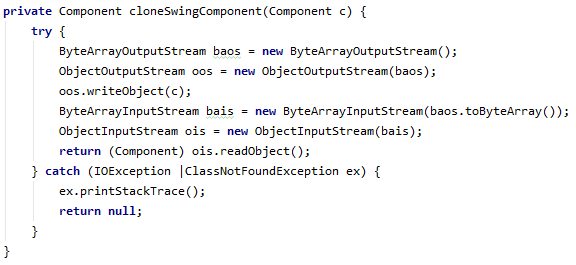
\includegraphics[width=100mm]{copy_constructor.png}
                \caption{Some caption of the constructor.}
            \end{figure}
        
            Upon completion of cloning the button blocks available to the user on the button panel,
            the user will need the ability to edit what's inside the print button to their choosing.
            I implemented a simple window to popup to the user, whereby the user can enter what they
            wish to be printed.

            \begin{figure}[h]
                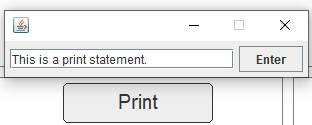
\includegraphics[width=50mm]{print_statement1.png}
                
\includegraphics[width=50mm]{print_statement2.png}
                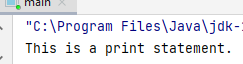
\includegraphics[width=50mm]{print_statement3.png}
                \caption{Ability to create a print statement block, with a text of the users' choosing,
                and successfully print it out to the console.}
            \end{figure}

        \clearpage
        \subsection{DragLayout \& ComponentMover}
            It is a key objecive, although it may not be explicitly noted in this report, but
            it is implied, that when designing a project such as this that the user has, not only
            to be able to interact with the features the program provides, but be able to edit these
            features - one way being through movement. The user will need access to drag
            components around to their desirable positions. \textit{Rob Camick's} blog on this specific
            feature provides a \texttt{DragLayout.java} class file that does exactly that, and it is
            paired up with another class file \texttt{ComponentMover.java}. Both classes are dependent
            on eachother to work~\cite{dragLayout}. The decision was between using a null layout or a drag layout manager.
            The answer is drawn from the 3 different functions a manager performs:

            \begin{itemize}
                \item sets the locations of the components in the container.
                \item sets the size of the components in the container.
                \item calculates the preferred size of the containter.
            \end{itemize}

            A null layout is a layout that technically it's a legitimate layout manager. This means that
            no layout manager is assigned, meaning the components can be put at specific \texttt{(x,y,z)}
            coordinates. It can be particularly useful for making quick prototypes but that is essentially it.
            When dragging components inside a JPanel container, it should be clear that the manager
            should not replace the location of the component. That being said, there's no reason a layout
            manager could \textit{not} set the size of the objective to calculate the preferred size
            for the container. Essentially, the \texttt{DragLayout} manager was designed to replace
            a null layout. \\
            
            The manager uses the \texttt{ComponentMove.java} class to drag the objects.
            \texttt{DragLayout.java} is just the foundation - it is not responsible for the moving
            of any components. One could use a \texttt{mouseListener} to handle the \texttt{mousePressed}
            event to track the original location of the component, followed by a \texttt{MouseMotionListener}
            to handle the \texttt{mouseDragged} event so the component can allow itself to be moved via
            each drag event. However once tested, I notice this was producing flickering results on the
            components that I was trying to move on the drag layout. This wasn't appealing and rather
            distracting instead, the user's experience would decline as a result. \texttt{ComponentMover.java}
            gives us the flexibility for controlling which component is responsible for moving a window
            \cite{componentMover}.

            \clearpage
            In regards to my action listener events, when a button on the side panel is clicked,
            it's going to do the same process every time, no matter what button is being
            clicked. It would be lazy to create action listener events for every single button
            to do the exact same process. Thinking ahead for when I add future buttons to the
            side panel, I decided to create an action listener variable so that all the buttons
            can call this single event instead creating the same event for every button. \\

            \begin{figure}[h]
                \centering
                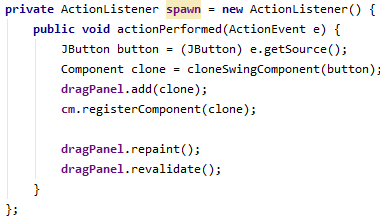
\includegraphics[width=120mm]{actionlistener.png}
                \caption{Creating the action listener one time and one time only to be used for all
                the buttons.}
            \end{figure}
        
        \clearpage
        \subsection{Deleting blocks}
            An important objective for the user is the ability to edit their programs. This includes
            deleting blocks they have made by mistake/no longer want anymore. There isn't any
            sense in having the user close and re-open the application each time they need to
            delete a block as this would also clear all their progress. This isn't smart.

            There are several concepts to think about when implementing this. Key questions to
            ask include \textit{what will I use to delete a block} and \textit{how will I use this
            to go about deleting the block}. There are many ways to go about this, one being that there
            may be a recycling bin in the corner, where the user would be able to drag their blocks over
            there and drop them, causing the blocks to be deleted in the process. App Inventor uses this
            method, and Scratch uses a method where you drag the blocks back into the block palette on
            the left hand side - where the blocks are to create your program - and this would cause those
            blocks to be delete too. Both works with stacks of blocks too if they are interconnected. \\

            Both current methods work and sound great - however I want to be a bit more simple than that.
            My plan is to setup a new java class that deals specifically with deleting blocks. This class
            will extend the \texttt{MouseAdapter} library - this library will be the answer as it holds
            the functions that allow me to read mouse clicks - such as two specific functions that I will
            override: \texttt{mousePressed} and \texttt{mouseReleased}.

            Using these two functions together, I can detect the mouse clicks on the button and use these
            to delete a button. How so? By use of the right click button. Currently, the user has no
            reason to use the right click mouse button as it serves to purpose - this is about to change.
            The user will be able to right click any block, resulting in deletion. This will work
            dynamically at runtime, so the user will not need to restart the application.
            \texttt{mousePressed} will become true when a mouse click has been pressed, followed by the
            function \texttt{mouseReleased} which will confirm the press and a new condition if that press
            is a right click - if so then it will proceed to remove the button and update the panel. Finally,
            all that's left is for me to call this class on the clones that are created, a simple one line. \\

            Figures 14-17 illustrate my point in practice, note this this instance is performed all at
            runtime, hence the proof via console screenshots showing each program being run within the
            overall instance.

            \clearpage
            \begin{figure}[h]
                \centering
                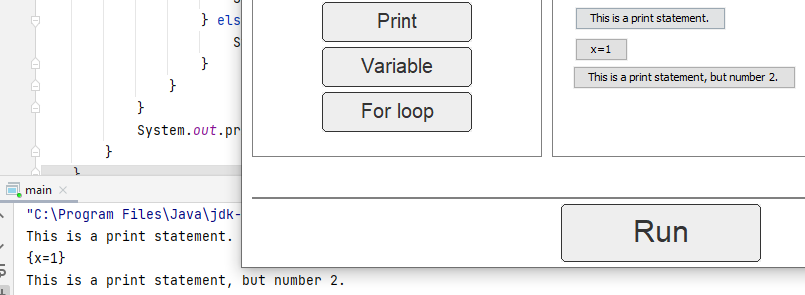
\includegraphics[width=120mm]{delete_block1.png}
                \caption{Two print statements and a variable initialised in a hashmap.}
            \end{figure}

            In Figure 15 I delete the first print statement and run the program again.

            \begin{figure}[h]
                \centering
                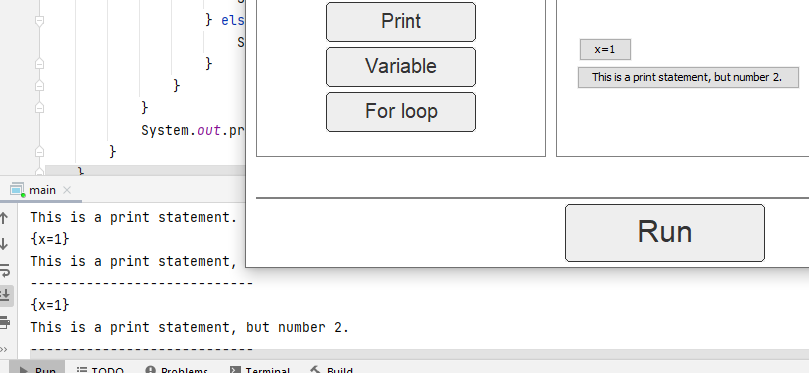
\includegraphics[width=120mm]{delete_block2.png}
                \caption{Deleting the first print statement and running the program again.}
            \end{figure}

            So far I have created three blocks, deleted one and the process has worked. To
            confirm, I am using the right click on the mouse in order to delete the component.

            \clearpage
            Further in Figure 16, I delete the variable and continue to run the program.

            \begin{figure}[h]
                \centering
                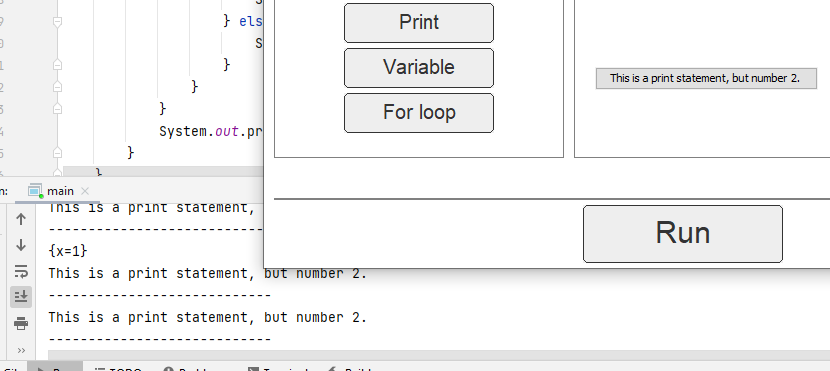
\includegraphics[width=120mm]{delete_block3.png}
                \caption{Deleting the variable and running the program, all working as intended.}
            \end{figure}

            Finally, I delete the final print statement. Programs cannot be run if there are no
            contents in the panel, thus I create a new statement, and run this too.

            \begin{figure}[h]
                \centering
                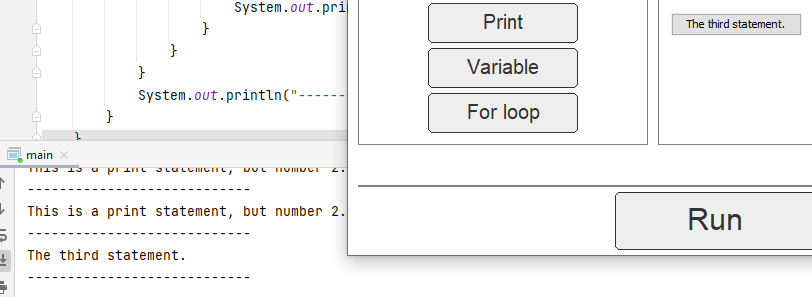
\includegraphics[width=120mm]{delete_block4.png}
                \caption{Deleting the final print statement, and reintroducing a new one!}
            \end{figure}

            I now have a fully functional deleting mechanism allowing users to edit and change
            their work as they go.

        \clearpage
        \subsection{Maintaining order of the program}
            A crucial objective to be fulfilled in this project is the flow of the program and ensuring
            that where the user places their blocks determines its position in their program and
            how they are interacted at compile time. It is key that if the user declares an assignment
            variable, followed by a print statement in their program printing the variable, that when
            they proceed with the \texttt{Run} button, there is a mechanism behind the scenes that will
            maintain a block structure. So when the print statement is met at run time, it understands
            what it is trying to print out, and where to get it from. Maintaining this block structure
            enables the user to create high level programs and begin thinking about their programs
            syntactically, which will help them develop skills for writing code in text-based languages. \\

            I used the \texttt{Collections} and the \texttt{Comparator} library to achieve this. Using these libraries
            together, I was able to interact with the data structure instantiated by collecting the components
            of the panel in an arraylist of type \texttt{Component}. Using the latter library, I compared
            the Y coordinate locations of all components in the arraylist and sorted them based on that
            rule - however if it is apparent that there are several components with the same Y coordinate,
            then they are further sorted on their X coordinates. \\

            Below in Figures 18-21, we can see how the methods I have discussed work in practice. The console
            in Figure 18 console reveals to us the block structure working as intended, sorting by their Y
            coordinate. \\

            I would also like to point out that on my end as the developer, this entire program is being run
            in one go live at runtime! This is impressive and useful; if I wanted to I could, after full
            completion, export the program as an executable \texttt{.exe} file that users can use by opening
            it and letting the program run. Users are able to run their own program via the execution button
            \texttt{Run} and this would work live for them as each time they run their own programs, it is
            being updated and runs with any changes they have made.

            \clearpage
            \begin{figure}[h]
                \centering
                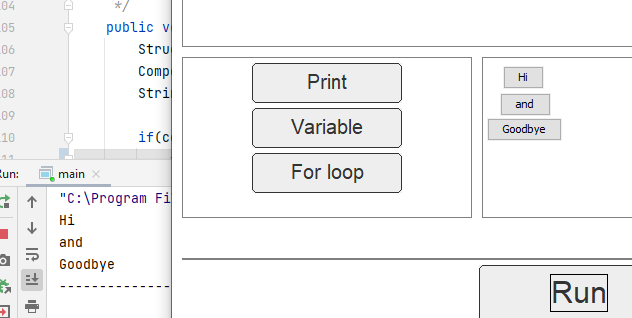
\includegraphics[width=120mm]{blockstructure1.png}
                \caption{Normal block structure being sorted by their Y coordinates.}
            \end{figure}

            In Figure 19, I reajust the program, moving one block further to the right but above the
            \texttt{Goodbye} print block. Running the program again also updates the block structure
            accordingly and correctly, sorted by their Y coordinate as main priority.

            \begin{figure}[h]
                \centering
                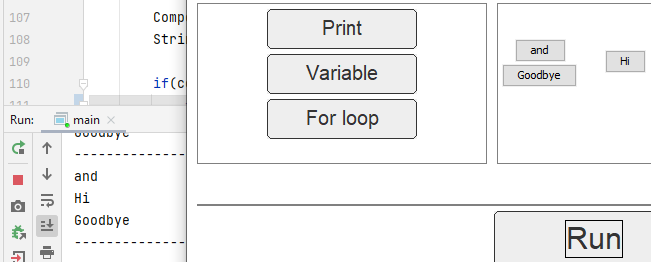
\includegraphics[width=120mm]{blockstructure2.png}
                \caption{\texttt{and} print statement is classed as the first element
                in this program.}
            \end{figure}

            Figure 20 proves how when aligning all of the blocks by their Y coordinates, that their X
            coordinates are then learnt and used to determine their knew positions. Note that if their
            X \& Y coordinates are identical, then the block that was instantiated first will take priority.
            Although it would not be ideal as a programmer to have blocks hidden on top of one another.

            \clearpage
            \begin{figure}[h]
                \centering
                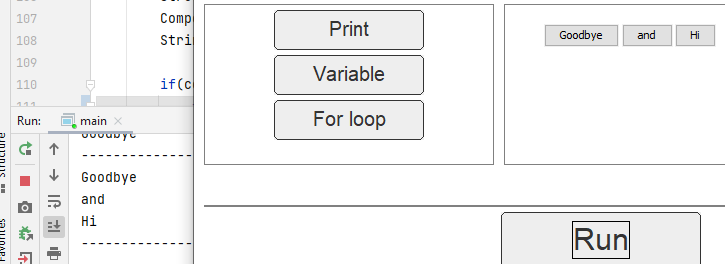
\includegraphics[width=120mm]{blockstructure3.png}
                \caption{All Y coordinates are the same so they are sorted by their X coordinate.}
            \end{figure}

            Furthermore in Figure 21, continuing from Figure 16, if I were to move just a few of the
            blocks up immediately, the block structure updates again and works as intended.

            \begin{figure}[h]
                \centering
                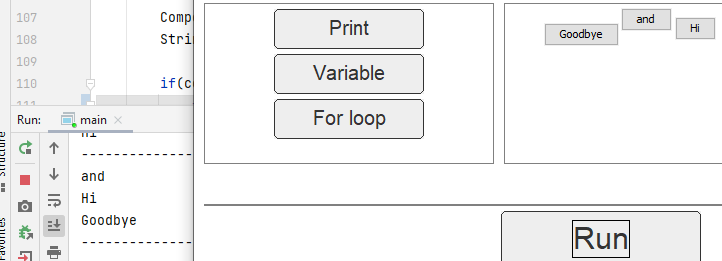
\includegraphics[width=120mm]{blockstructure4.png}
                \caption{In relation to Figure 20, if we adjust their Y coordinate, it will update
                its block structure.}
            \end{figure}
            
            Now I have a fully working block structure, capable of allowing blocks to be placed in a
            syntactical manner that holds true as with almost any other programming languages' structure.

        \clearpage
        \subsection{Console Output}
            Earlier in the report I discussed about the means to which the user would be able to 
            read their program outputs in a particular way, whether this be through a new window
            that would pop up as they ran their program, or perhaps a new side panel dedicated to
            a console output, similar to how Google's Blockly present how the user's blocks are
            represented in textual code in a side panel. I think it's a given why this is a necessity
            for this project or would purpose would it serve. Users will be able to learn what they
            are producing through the console and this console will work live in runtime, where each
            time they run their program, their console will run - similar to how the console works
            in Java.

            Figure 22 below shows an updated sketch of Figure 9 about how I intend to present the
            application to the user, with the console fitted. As you can see the console fits neatly
            along the right hand side of the program, showing clear output directly in front of
            the user. Obviously it is not for me to conclude whether this is ideal or not, hence why
            I will be asking my housemate for his permission on his opinion about the project and
            whether he finds it appealing or not.

            \begin{figure}[h]
                \centering
                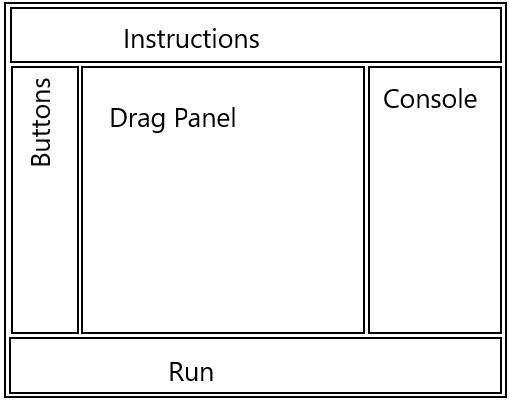
\includegraphics[width=110mm]{design_updated.png}
                \caption{Updated sketch of Figure 9, representing the new design for the program.}
            \end{figure}

            I will make a new Java class for the console. The implementation will consist of a \texttt{jTextArea}
            to represent the textual output of the console, rather than the even older API, \texttt{textArea}.
            The former API was developed after the significant issues that had come about with the latter,
            and it can be used within a \texttt{JScrollPane} so that it's content can extend beyond the
            bounds of its layout, with a horizontal and/or vertical scrollbar, incase output is too long
            in either direction~\cite{jTextArea}. Finally, I will place the scroll pane within the panel, which
            is placed within the border layout of the frame. That should complete the design side. \\

            However, I ran into an issue where there was a border between the edge of the panel and the text area. I thought
            that perhaps this was an issue with the border layout that I instantiated inside of the panel itself,
            since the panel is also being controlled by a border layout by the initial frame, so it's sort of like
            \textit{borderlayout-ception}. This was not the case. After researching the issue, I came to a
            resolution, and that the problem occuring here is that there is a border for not only the scroll pane,
            but for the text area too - thus I am seeing two different borders. To resolve this manually casted the
            border of the scroll pane to \texttt{null}, removing it and therefore fixing the problem.

            By placing the text area inside the scroll pane, followed by adding the scroll pane to the panel
            with a layout fixes the size. The layout I'm using is a border layout for the specific console
            pane, but this means that if I resize the program, or no matter how full the text area is,
            the text area adjusts to its surroundings and fills the size of the panel accordingly, leaving
            no padding or no borders that look unappealing and unnatural. \\

            In practice, Figure 23 shows how my console fits in my program, and how it works with
            any blocks that the user uses to programs. This is an excellent addition into the software
            and easy for all users to see. Right there in front if them, users do not need to look/check
            elsewhere to find where their programs are being outputted to. The scroll pane is a success
            as any strings too long in length, or any programs running too wide in height will all be
            accessible to the user via the scrollbars that will be readily available only when needed.
            
            \begin{figure}[h]
                \centering
                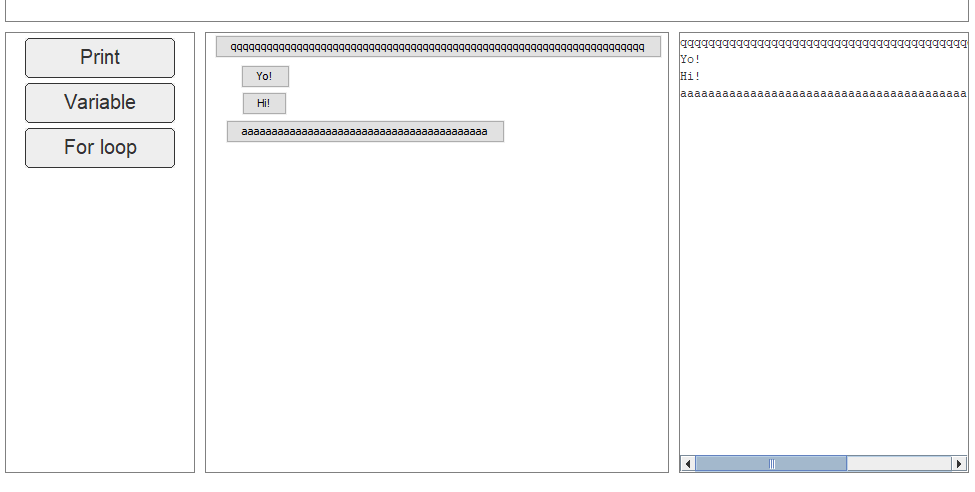
\includegraphics[width=160mm]{console.png}
                \caption{Console on the newly created right hand side panel.}
            \end{figure}
          
        
        \clearpage
        \subsection{Parser}
            It's time to develop the application and make it more sophisticated. At this current stage, all
            the user can do are print statements and create variables. The next big hurdle is the ability
            to interact with these variables that they have created. So for instance if the user has
            initialised a variable of \texttt{x=3}, then they would be able to create a block, with an
            expression \texttt{x+3} and result in a console output of \texttt{6}. This would be developed
            further to work with several variables. If initialised before hand, the user may also be able
            to interact with several variables, perhaps performing expressions such as \texttt{x*y}. \\

            To begin however, I think it's important to go back to our code and see if we can make anything
            a bit more abstract to make our job easier in terms of parsing the expressions. If the user is
            going to write the expressions in the print blocks, I would need to parse the print blocks each
            time to check whether what is written is an expression or just a regular statement. However,
            this leads to complications. In regards to printing a sentence, it's perfectly legal for
            users to write meaningless expressions as a sentence. Furthermore, it's also legal for users
            to include names that may so happen to be the name of their variable too, within their print
            blocks as a sentence without actually parsing that name as a variable. They could be referring
            to said variable instead. This seems far too complex to program into one simple button, and
            I think it's a wise decision to make this more abstract and separate what they can and can't do
            into different buttons. The print block will remain as a statement that will just print strings,
            but creating a new block that can be used for the user to only use as expressions is a more
            dynamic approach that I want to persevere. As a result this allows me to use a specific JButton
            function called the \texttt{setActionCommand}. Currently as I run the program, I would need to
            parse the text to determine what the button is. However, using this command I can set strings
            associated with each button, so with a print button I can label this an action \textit{print},
            with variables \textit{variable} and so on. This abstract refactor is smart for simple reasons.
            One being that if the user just wants to print out a statement, then if they're using a print
            block, I can simply write a condition where if the block is of action \textit{print} then simply
            print this out. That is the user's intention after all, I don't need to parse it and check for
            special characters such as \texttt{=} incase the user is trying to assign a variable and so forth.
            Users may want to use special characters and/or their variable names as a print statement, and
            should do so freely. \\

            Below in Figure 24 I have created the new button that will be used for interacting with variables
            through basic methods such as arithmetic expressions, called \texttt{Expressions}. This will
            have its own action set to it, which allows me to be more flexible in the code. When this
            button is pressed, I understand what the user is trying to do and I can begin implementing the
            functionality that will be used to calculate the expressions that the user is attempting to
            solve. This is practical, knowing what the user is doing at runtime rather that trying to
            deciper what the user is thinking.
            
            \clearpage
            \begin{figure}[h]
                \centering
                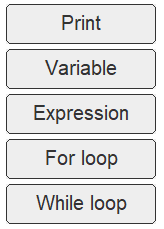
\includegraphics[width=20mm]{updated_blocks.png}
                \caption{The next blocks available to the user in the button panel. Note that the
                \texttt{For} and \texttt{While} loop blocks are not functional and simply there
                for display to show what the button panel is designed to look like.}
            \end{figure}

            Users need to be able to interact with variables. If a variable has been initialised,
            my program will need to parse the expression they use, and identify if what they are
            calculating a variable, or an arithmetic expression of numbers, or numbers against
            variables. As a result, I will only be interacting with variables names of length
            1 character. This is just a simple use case for now, that can be developed in future
            work to allow variable names of any length. With a variable name of 1 character, I can
            evaluate expressions each token at a time, so an expression of \texttt{1+2} has a total
            of 3 tokens. Through this evaluation I can judge each token and decide whether the token
            is a number, a character - and if so, a variable that exists - or an operator. I am
            creating new classes for all the different tokens, such as for the operators - addition,
            subtraction and so forth, as well a class for variables, a class for numbers and a parser
            class which will parse the tokens in the expression and use their respective sub classes. \\

            For basic simple arithmetic expressions such as \texttt{1+2}, my program is parsing this
            expression firstly by identifying the first token, which is a number. I start to build a
            string around this, scanning for the next token which is an operator, continuing the string
            and scanning for the next token which is another number. After scanning one last time and
            finding \texttt{null} or and empty byte, the string is built and we continue on to the
            operator process - what operator is it? Through simple conditionals, I can check the equality
            of the operator against the four different operators and those that match will then perform
            the equation using the numbers inherited from their own class. The equation is evaluated and
            the result is returned ready to be printed out.

            \begin{figure}[h]
                \centering
                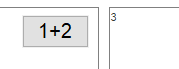
\includegraphics[width=56mm]{1+2.png}
                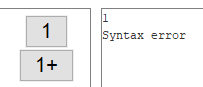
\includegraphics[width=50mm]{1+.png}
                \caption{The expression \texttt{1+2} in full effect, as well as just a single digit
                expression, and an expression that is half completed printing out an error for the
                user to see.}
            \end{figure}

            \clearpage
            In regards to interaction with variables, the parser works the same. After scanning a
            token, if said token happens to be a character, this token is searched up in the hashmap
            I created where variables are stored alongside their values. If the variable is found,
            their value is returned. If this variable is not found, a key exception is thrown,
            printing an error to the user in their console that the so called variable does not exist.
            This is also effective for variables that are initialised with the value of another variable
            beforehand and vice versa. Figure 26 shows the parser working in full action, alongside
            a small program I \textit{blockingly} created.

            \begin{figure}[h]
                \centering
                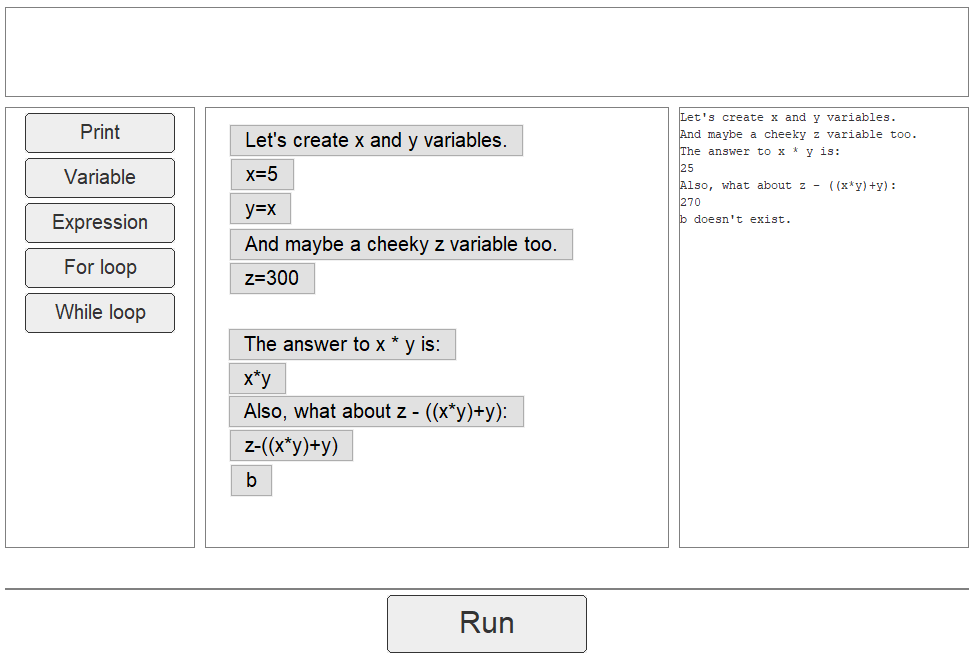
\includegraphics[width=170mm]{working_interpreter.png}
                \caption{The interpreter working and fully functional as it parse's the user's
                expressions and understands where to find the necessary variables and
                what values are assigned to them.}
            \end{figure}

            I now have a fully working parser in my project which finally means this project
            is a little bit more sophisticated than what it used to be! Although this was definitely
            the most challenging part of the project thus far and took up far more time than I
            had planned, it's great to finally see the complexity of the project shining.


        \clearpage
        \subsection{For Loop}
            The next challenge I am faced with are the loops to be performed. Loops are an essential
            part to programming that all beginners must be aware of learn in order to make good
            practice with the features available to them when working on any project. Loops in
            computer programming are important that they can perform tasks within seconds while
            reducing, to a great extent, time and efforts of the users~\cite{loops}. Without loops,
            beginners will just be programming in a linear manner and will miss out on the fundamentals,
            which in turn will help develop their problem solving skills. \\

            The important part to focus and make sure I get correctly is how the for loop will
            function with the blocks that follow. It was a decision between thinking about making
            blocks connect to the for loop, or designing a for loop block that has a wide body and
            blocks can fit inside it. These different issues can take up a lot of time thinking
            about and attempting to implement, so to keep it simple, a foundation to this problem
            would work sufficiently. The functionality of the for loop will work by scanning for
            the next block that follows, and only applying the for loop to that block. This is
            a basic infrastructure that can be developed in the future but will still serve as
            a loop that users can use and learn from effectively. \\

            In Figure 27, the following program works using 3 print statements, and a for block.
            The for loop block is currently always set from 1 to \textit{x} amount of times that
            the user is able to enter. For demonstration purposes, I have entered an amount of 10,
            and ran the program, showing the for loop in practice, revealing that it is working
            accordingly and can be used to loop statements and/or expressions. This is just the
            beginning but this will be worked on in future work.

            \begin{figure}[h]
                \centering
                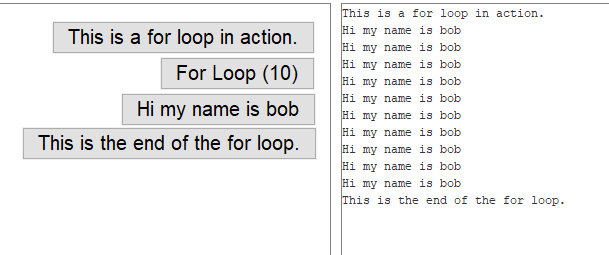
\includegraphics[width=130mm]{for_loop.png}
                \caption{For loop block in action using the next block as it's body, looping
                it 10 times as indicated by the block.}
            \end{figure}
        
    \clearpage
    \section{User Feedback}
        This section of the report involves feedback from one user, being my housemate. I have asked for
        their permission and requested if they would like to take part and simply share their opinion on
        the project. My housemate would use the program for fifteen minutes, and I handed them a task sheet
        to complete the following tasks:

        \begin{itemize}
            \item print out a sentence.
            \item create a variable of any value.
            \begin{itemize}
                \item use an expression to multiply this variable by 5.
                \item create another new variable, assigning it to the previous variable you have made.
                \item subtract the new variable by 1000.
            \end{itemize}
            \item loop a statement and/or an expression 100 times.
        \end{itemize}

        The user had no difficulties completing the following tasks. The instructions located at the top were
        easy for them to follow, completing the tasks with ease. The user hesitated when it came to the task
        of the for loop, but quickly caught on from re-reading the instructions that the for loop currently
        only loops the next consecutive block. All tasks were completely without any problems. \\

        Afterwards, I let the user explore the remainder of the time and share their thoughts. Overall, the
        user reacted positively towards the compact but tidy layout of the program, with the console on the
        right hand side being a fantastic feature that works dynamically with the programs they create. The
        instructions at the top were just written out in a long sentence and the user suggested perhaps
        formatting the instructions, making them larger and a less compact so it's not like a block of text.
        The user also pointed out the following when initialising a variable of \texttt{a=5}, and performing
        the expression \texttt{a/2} which printed out 2. All results are returned as integers hence why this
        had not returned a decimal. This will be a note for future work to return to this part of the project
        and develop the implementation further to allow float types to be returned, as well as long types
        incase the numbers are too large to store in an integer type.

    \clearpage
    \section{Conclusions \& Evaluation}
        A majority of the challenge and complexity that this project yielded comes from the
        involvement of meta-programming and of handling unbounded user input. Combined, these
        two practices have a significant impact to increase the possibility of mistakes and
        problems appearing. In closing, I would consider this project to be a success - most,
        if not all, of the primary objectives have been met. A program has been made to
        ultimately serve as an alternative, I would argue a more simple approach, to the
        current graphical programming languages out there, namely Scratch \& MIT App Inventor. \\

        I have learnt a lot from this project, especially the Java Swing API and what it is
        capable of creating. Skills I have learnt during my degree I put to practice in this
        project, such as time management in regards to Software Engineering, keeping to an
        agile plan and having regular meetings with my supervisor, as well as compiler design
        and building a parser. One feature in particular that I learnt was the debugging feature
        in the IDE I was susing - IntelliJ. This feature helped me debug any errors I had
        throughout the program, in particular why my variables weren't being stored into the
        hashmap, or why my parser wasn't looping through the entire expression properly. Both
        issues were resolved through the debug feature - revealing that I had an infinite loop
        in my parser which was why it wasn't looping through the expressions correctly.
        To add on, not only have I learnt from this project but I have almost definitely
        improved my ability to problem solve, and program at a higher level than what I could before,
        learning to refactor and remove redundant code, as well as make code more abstract to work
        in larger projects more efficiently, meaning less lines of code and more functions work
        with one another. \\ 

    \subsection{Requirements}
        In section 4 of the Requirements Analysis, 4.1 in particular shows the mandatory
        requirements that were to be met for this project to be fully complete and functional.
        From the 7 requirements, all were met apart from half of the fifth requirement -
        \textit{The user shall be able to use functional loops such as for and while loops}.
        I have a basic implementation of the for loop functional, but not as complex as it can
        be. As for the while loop, I have not implemented this at all. The basic infrastructure
        for this project to evolve to become more sophistcated was the challenging part and
        took a lot longer to complete than I aimed for, but it is complete. The infrastructure
        was the most important part of this project however. Now that this is completed, for
        future work I can continue to fully complete the basic features I have implemented,
        as well as continue to work on new features that work around the infrastructure I have
        finally created. As for the desirable requirements, in terms of editing, part of those requirements were
        met too. The ability to delete blocks dynamically allows the user to freely edit their
        work without having to restart the application. The rest of the desirable requirements
        can also be met in future work after this report.

    \subsection{Future Work}
        I will be continuing this project after this report is complete. I want to embellish
        the project, perhaps with some colour coded blocks, making it look less bland overall.
        This is matching the desirable requirements that I stated in section 4.2. Before that,
        I will work on improving the for loop and making it more functional working with
        several blocks instead of just the next block. The while loop will be implemented
        to work with conditional statements, as well as including booleans, \texttt{True} and
        \texttt{False}. Booleans will be a great addition as this will also provide functionality
        with creating conditional \texttt{if} statements that the user can do to run certain
        blocks given certain conditions are met, resulting in their own programs becoming
        more complex and sophisticated. So to summarise, I want to continue working on the
        mandatory requirements, developing the existing features and working on implementing
        the while loop. Such developments also include variables - in particular the ability
        to have variables names of any length. Currently variables are of just 1 character,
        but I want to abstract this and have variables names of any length allowing users to
        use more meaningful variable names than just single characters. \\

        In regards to the user feedback, I will definitely continue working on the design layout
        and making it more appealing and more \textit{comfortable} since currently it is a bit
        compact currently. Furthermore, all expressions are returned as integers, rather than
        the correct result, which may be a long and/or a float type. I can work on embellishing
        this implementation too and working on enabling users to interact with more results than
        they currently can.

    
    \clearpage
    \section{Appendix}
        \subsection{Interim Log}
            \textbf{Friday 23\textsuperscript{rd} October}
                \begin{itemize}
                    \item Discussing what my key interests are.
                    \item Deciding which projects are suitable for me.
                    \item Showing me some of my supervisor's projects. 
                    \item Going through the introduction of the project proposal. \\
                \end{itemize}
            \textbf{Monday 9\textsuperscript{th} November} 
                \begin{itemize}
                    \item Focusing on time management between project and university
                    studies.
                    \item Strong introduction, that explains what I'm doing!!
                    \item Project proposal:
                    \begin{itemize}
                        \item deeper detailed objectives.
                        \item be more specific if I can.
                    \end{itemize}
                    \item grouping objectives into one group, not several.
                \end{itemize}

    \clearpage
        \subsection{Project Log}
            \textbf{Saturday 16\textsuperscript{th} January}
                \begin{itemize}
                    \item Meeting after Christmas break.
                    \item Motivation to start the project.
                    \item Planning how to being the project. \\
                \end{itemize}
            \textbf{Monday 15\textsuperscript{th} February}
                \begin{itemize}
                    \item Basic GUI completed and shown.
                    \item Discussing the next steps, side panels.
                    \item Begin with two panels, buttons on the left hand side. \\
                \end{itemize}
            \textbf{Monday 22\textsuperscript{nd} February}
                \begin{itemize}
                    \item Panels completed and shown.
                    \item Print button created in side panel.
                    \item No interactivity yet.
                    \item Deciding how I plan to spawn the buttons after they are clicked,
                    or dragging them onto the main panel. \\
                \end{itemize}
            \textbf{Wednesday 3\textsuperscript{rd} March}
                \begin{itemize}
                    \item No further improvements to the project.
                    \item Talking about what I'm stuck on, how to go further.
                    \item Have I done any of this before? Check through my further programming
                    work from First Year. \\
                \end{itemize}
            \textbf{Wednesday 10\textsuperscript{th} March}
                \begin{itemize}
                    \item Made some further progress on the project.
                    \item Click the buttons on the side panel to clone them and spawn
                    them on the main panel.
                    \item Also implemented a drag class that deals with dragging the components
                    on the main panel, some interactivity! \\
                \end{itemize}
            \textbf{Monday 19\textsuperscript{th} April}
                \begin{itemize}
                    \item Not much progress made. Tidied current implementations up a bit.
                    \item Discussed current mental situation given the certain circumstances.
                    \item Implemented variables that are stored in a hashmap with their value.
                \end{itemize}
            \textbf{Thursday 22\textsuperscript{nd} April}
                \begin{itemize}
                    \item Data structures! Working on the parser, explaining and helping me
                    understand the fundamentals of the infrastructure needed to interact with
                    variables.
                \end{itemize}
            \textbf{Monday 26\textsuperscript{th} April}
                \begin{itemize}
                    \item Sorted the components on the main panel.
                    \item Procedural order of programming is maintained - components are organised
                    by their Y-coordinate, and if they're equal they are ordered by their X
                    -coordinate. \\
                \end{itemize}
            \textbf{Wednesday 5\textsuperscript{th}May}
                \begin{itemize}
                    \item Showed off all my current work completed. A parser that interacts with
                    variables and print statements, as well as expressions to calculate variables
                    or just perform arithmetic expressions.
                    \item Talking about implementing a basic for loop to have a foundation for
                    full funtionality to be completed in future work.
                \end{itemize}

        \clearpage
        \subsection{Project Proposal}
            \textbf{Motivations} \\\\    
            The motivation behind this project it that it will push my Java programming
            skills to limit, and experience designing software for other people rather
            than just for my own benefit. This will help me put my focus on the user's
            goals rather than my own. Additionally, I can put this project on my portfolio
            to show future employers!

            This project will further put content learnt from modules in my degree to                practice. Time management techniques from Software Engineering will help me
            manage when and what I should be focusing on. Furthermore, concepts learnt
            from Human Computer Interaction will aid me in focussing on user design for
            the user's goals; implementing a user interface that everyone will be able to
            use effectively.
        
            Finally, the ability to use Java this extensively will most definitely improve
            my proficiency of the skill! \\\\
            \textbf{Aims} \\\\
            The aim of this project is to design and implement a user friendly interface for
            the user to graphically program basic functions. Simple functions may include:
            \begin{itemize}
                \item loops.
                \begin{itemize}
                    \item this includes \texttt{for} and \texttt{while} loops.
                \end{itemize}
                \item conditional statements, such as \texttt{if} statements.
                \item variables!
                \item arithmetic expressions.
                \item print statements.
            \end{itemize}
            
            This is necessary as it provides another programming viewpoint for the user,
            which can aid them understand the process and flow of how said program may be running.
            It is also friendly and less intimidating for newer users, relative to a textual/command
            line script.
                
            I am going to program this is Java, my most experienced language, making use of Java's
            smart GUI design feature, whilst learning and building knowledge on said feature for my
            own experience. \\\\
            \textbf{Objectives} \\\\
            The main objectives are:
            \begin{enumerate}
                \item To investigate system requirements and produce a requirements specification.
                \item To select and justify an appropiate research design for the project.
                \item Implement a simple user-friendly interface which is easy to use.
                \item Functional and working loops, conditionals that can be interacted
                with. \\
            \end{enumerate}        
            \textbf{Exta Objectives}
            \begin{enumerate}
                \item Colour coordinate the different functions.
                \begin{itemize}
                    \item for instance, the loops and conditionals can be coloured differently to show more
                    clearly what they represent.
                \end{itemize}
                \item Implement an undo button.
                \item Implement a redo button.
                \item Testing by a regular user, of the software.
            \end{enumerate}
            \textbf{Relevance} \\\\
            This project involves modules across my degree, as well as Java; the most extensively
            used language across my university education thus far. This project will use skills learnt
            in Human Computer Interaction; test my ability to understand the user's perspective and
            struggles, involving the evaluation of the software, rather than my own when designing
            the interface for them to use.
        
            This project also incorporates key concepts understood from Software Engineering.
            The ability to criticse my own work, collect requirements, manage time and manage an
            agile approach to the project. Therefore, this project will test my ability to make use
            of several skills in such a way that they will be used outside of my university education. \\\\
            \textbf{Resources Required} \\\\
            None. \\\\
            \clearpage
            \textbf{Personal Timetable}
                \begin{figure}[h]
                    \centering
                    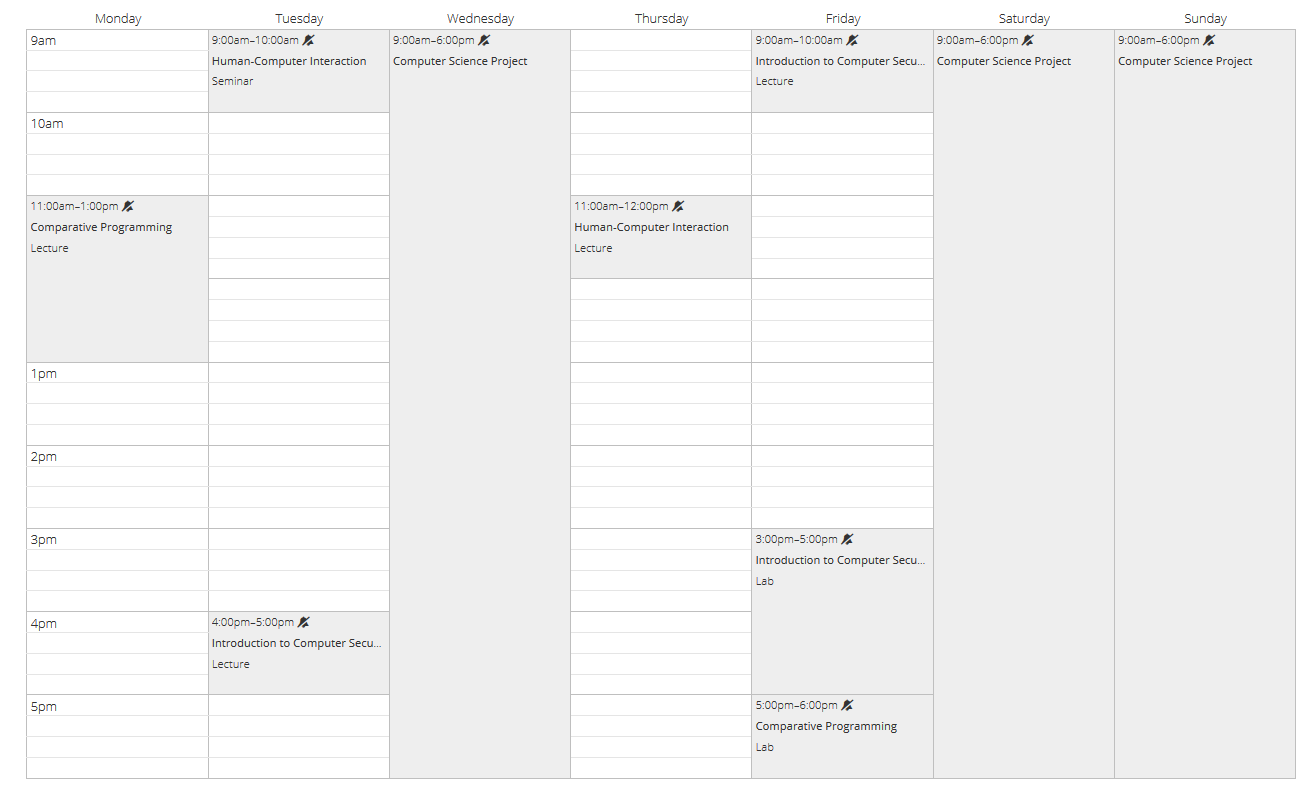
\includegraphics[width=175mm]{timetable.png}
                \end{figure}    

    \clearpage
    \printbibliography
\end{document}